\section{ Gaussian Processes}	\label{sec: GP-2}

This chapter presents Gaussian processes (GPs), which play a key role in this thesis. They can be used for classification and regression problems, Regression is the one that is more important in the context of control. For this reason, Gaussian process regression in the realm of control systems is presented in detail, where Section \ref{sec:section2.1} describes the method based on linear functions and Section \ref{sec:section2.2} extended to non-linear functions. In Section \ref{sec:section2.3}, the focus shifts to long-term prediction using Moment Matching Approximation. Here, the capability of prediction to provide predictions over extended time horizons is explored, which is crucial for effective control strategies that require anticipation of future system behavior. Finally, Section \ref{sec:optimize_hy} delves into GP hyperparameter optimization, elucidating techniques for fine-tuning the parameters of Gaussian processes to enhance their predictive performance. This section highlights the importance of parameter optimization in maximizing the utility of GPs within control systems.

\subsection{Linear Regression Model}\label{sec:section2.1}
In the realm of machine learning algorithms, Gaussian processes are often used for supervised learning, i.e., labeled input-output data is used to determine a mapping between input and output (see \cite{lawrence2005} for an exception). Probabilistic regression is usually formulated as follows: given a training set $D = \{(\mathbf{x_i}, y_i), i = 1, \ldots, n\}$ of $n$ pairs of (vectorial) inputs $\mathbf{x_i}$ and noisy (real, scalar) outputs $y_i$, compute the predictive distribution of the function values $f^*$ (or noisy $y^*$) at test locations $\mathbf{x^*}$. In the simplest case (which we deal with here), we assume that the noise is additive, independent, and Gaussian, such that the relationship between the (latent) function $f(x)$ and the observed noisy targets $y$ is given by:
\begin{equation}\label{eq:latent_function}
\begin{aligned}
    f(x_i) &= \mathbf{x_i}^T \mathbf{w}, \, \, \,\, \, \,\,\, \,\,\,\,\,\,\,\,\, \, y_i &= f(\mathbf{x_i}) + \epsilon_i
\end{aligned}
\end{equation}

where $\mathbf{w} \in \mathbb{R}^D$ is the weight column vector of the linear model, $\mathbf{x}$ is the input vector,  $\epsilon_i \sim \mathcal{N}(0, \sigma^2_{\text{noise}})$, and $\sigma^2_{\text{noise}}$ is the variance of the noise and $y$ is the observed value.
The noise $\epsilon$ is assumed to be zero-mean with variance $\sigma^2_n$, thus $\epsilon \sim \mathcal{N}(0, \sigma^2_n)$ 

\textbf{Definition 1}: A Gaussian process (GP) is a collection of random variables, any finite number of which have consistent joint Gaussian distributions. It is a Bayesian approach that assumes a GP prior over functions \cite{quinnonero2007approximation}, i.e., assumes a prior that function values behave according to
\begin{equation}\label{eq:prior_function}
    p(f | x_1, x_2, \ldots, x_n) = \mathcal{N} (0, K(\mathbf{x_1}, \mathbf{x_2})), 
\end{equation}

where $f = [f_1, f_2, \ldots, f_n]^{\top}$ is a vector of latent function values, $f_i = f(\mathbf{x_i})$, and $K(\mathbf{x_1}, \mathbf{x_2})$ is a covariance matrix, whose entries are given by the covariance function, $K(\mathbf{x_1}, \mathbf{x_2})_{ij} = k(\mathbf{x_i}, \mathbf{x_j})$. The covariance function encodes our assumptions about the function we wish to learn by defining a notion of similarity between two function values, as a function of the corresponding two inputs. A very common covariance function is the Gaussian, or squared exponential\cite{williams2006gaussian},
\begin{equation}\label{eq:covariance_function}
    K_{ij} = k(\mathbf{x_i}, \mathbf{x_j}) = \sigma_f^2 \exp\left( -\frac{(\mathbf{x_i} - \mathbf{x_j})^2}{2l^2} \right),
\end{equation}
where $\sigma_f^2$ controls the prior variance, and $l$ is an isotropic lengthscale parameter that controls the rate of decay of the covariance, i.e., determines how far away $\mathbf{x_i}$ must be from $\mathbf{x_j}$ for $f_i$ to be unrelated to $f_j$. We term the parameters that define the covariance functions hyperparameters. Optimization of the hyperparameters based on data is discussed in Section \ref{sec:optimize_hy}.

\begin{figure}
    \centering
    \begin{subfigure}[b]{0.5\textwidth}
        \centering
        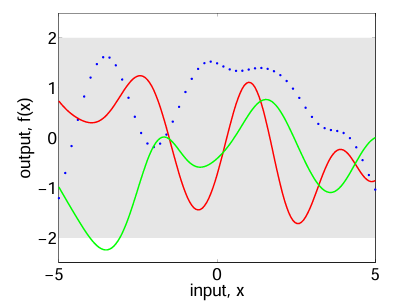
\includegraphics[width=1\linewidth]{figures/prior.png}
        \caption{prior}
        \label{fig:prior}
    \end{subfigure}
    \hfill
    \begin{subfigure}[b]{0.5\textwidth}
        \centering
        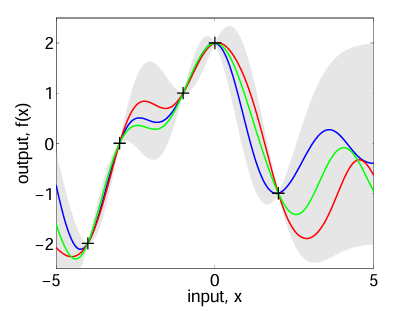
\includegraphics[width=1\linewidth]{posterior.png}
        \caption{posterior}
        \label{fig:posterior}
    \end{subfigure}
    \caption{Panel (a) displays three functions drawn at random from a GP prior. The dots represent values of \(y\) actually generated, while the other functions have been drawn as lines by connecting a large number of evaluated points.Panel (b) illustrates three random functions drawn from the posterior, i.e., the prior conditioned on the five noise-free observations indicated. In both plots, the shaded area represents the pointwise mean plus and minus two times the standard deviation for each input value (corresponding to the 95\% confidence region), for the prior and posterior, respectively \cite{williams2006gaussian}.}
    \label{fig:prior_posterior}
\end{figure}

\subsubsection{Posterior Distribution}
To predict function values for all inputs considering observations, the equation 
\begin{equation}
    f(X^*) = X^T_*\mathbf{w}
\end{equation} 
is used, where \( X^* \) denotes a matrix consisting of test points \( \mathbf{x^*} \) such that \( X^* \in \mathbb{R}^{D} \), \( X^* = [\mathbf{x^*_1, \ldots, x^*_s}] \). The posterior distribution of weights, denoted as $w$, is used to predict function values for all inputs considering observations. This distribution is obtained through Bayes' rule, where the posterior ($p(a|b)$) is proportional to the likelihood ($p(b|a)$) multiplied by the prior ($p(a)$) and normalized by the marginal likelihood ($p(b)$). In the context of the posterior distribution of weights, Bayes' rule can be rewritten as:
\begin{equation}\label{eq:bayes_rule}
    p(\mathbf{w}|\mathbf{y},X) = \frac{p(\mathbf{y}|X,\mathbf{w}) \cdot p(\mathbf{w})}{p(\mathbf{y}|X)}
\end{equation}

\begin{figure}
    \centering
    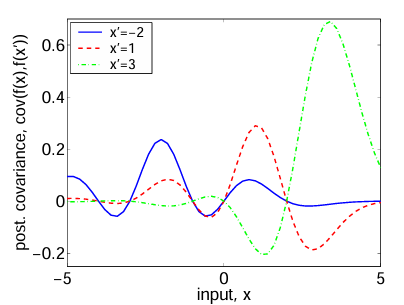
\includegraphics[width=0.6\linewidth]{figures/posterior_cov.png}
    \caption{The posterior covariance illustrates the covariance between \( f(x) \) and \( f(x') \) for the same data, with three different values of \( x' \). Notably, the covariance is high at points close to each other, diminishes to zero at the training points (where variance is absent due to the noise-free process), and subsequently becomes negative. This variation occurs because if the smooth function happens to be below the mean on one side of a data point, it is inclined to surpass the mean on the opposite side, resulting in a change in the sign of the covariance at the data points. In contrast, the prior covariance exhibits a Gaussian shape and remains non-negative. \cite{williams2006gaussian}.}
    \label{fig:Post_cov}
\end{figure}

The prior represents the model weights' beliefs without observations, often assumed as a Gaussian distribution with zero mean and covariance matrix as shown in Equation ( \ref{eq:prior_function}). The likelihood \( p(y | X, w) \) is the probability density function of the observations given the inputs and model weights, which can be determined using Equation (\ref{eq:latent_function}). 

\begin{equation}\label{eq:likelihood}
     p(\mathbf{y} | X, \mathbf{w}) = \mathcal{N}(X^T\mathbf{w}, \sigma^2_n I)
\end{equation}

By combining the prior Equation (\ref{eq:prior_function}) and likelihood Equation (\ref{eq:likelihood}), the posterior distribution of weights given observations  can be determined by their multiplication as shown in Equation \ref{eq:posterior}

\begin{equation}\label{eq:posterior}
    p(\mathbf{w} | \mathbf{y}, X) \propto p(\mathbf{y} | X, \mathbf{w}) \cdot p(\mathbf{w})
\end{equation}

The marginal likelihood is independent of \( w \) and just a normalization constant which does not influence the shape of the distribution. By substituting $A = \sigma^{-2}_n XX^T + \Sigma^{-1}_p$ and adding the terms $\pm \sigma^{-2}_n y^TX^TA^{-1}A^{-1}Xy \sigma^{-2}$ to the exponent, the equation can be rewritten as:
\begin{equation}
    p(\mathbf{w|y},X) \propto \exp\left(-\frac{1}{2} \mathbf{w}^T \left(\sigma^{-2}_n A^{-1}X\mathbf{y}\right) - \frac{1}{2} \sigma^{-2}_n y^TX^TA^{-1}A^{-1}X\mathbf{y}\right),
\end{equation}

where \( \alpha = \sigma^{-2}_n (A^{-1} y^T y - y^T X A^{-1}A^{-1} X^T y) \) is independent of \( w \) and hence also a scaling factor. Finally, the posterior is distributed according to:
\begin{equation}\label{eq:posterior_distrubtion}
     p(\mathbf{w | y}, X) = \mathcal{N}\left(\frac{1}{\sigma^2_n} A^{-1} X\mathbf{y}, A^{-1}\right)
\end{equation}



\subsubsection{Prediction}
When making predictions using Gaussian processes (GPs), incorporating observed data is crucial. For noise-free observations $\{(\mathbf{x_i}, f_i) | i = 1,...,n\}$, the joint distribution of training outputs $f$ and test outputs $f^*$ under the prior is given by:
\begin{equation}\label{eq:noisefree_joint_distrubtion}
    \begin{bmatrix}f, f^*\end{bmatrix} \sim \mathcal{N} \left(0, \begin{bmatrix} K(X,X) & K(X,X^*) \\ K(X^*,X) & K(X^*,X^*) \end{bmatrix} \right)
\end{equation}

To obtain the posterior distribution over functions, we condition this joint prior distribution on the observed data points. The resulting posterior distribution is expressed as:
\begin{equation}\label{noisefree_predictive_distrbution}
    f^* | X^*, X, f \sim \mathcal{N} \left( K(X^*,X)K(X,X)^{-1}f, K(X^*,X^*) - K(X^*,X)K(X,X)^{-1}K(X,X^*) \right)
\end{equation}

This enables sampling function values $f^*$ from the joint posterior distribution by evaluating the mean and covariance matrix.

Prediction with noisy observations incorporates additive independent identically distributed Gaussian noise. The joint distribution of observed target values and function values at test locations under the prior is given by:

\begin{equation}\label{eq:noisy_joint_distrubtion}
     \begin{bmatrix}\mathbf{y}, f^* \end{bmatrix} \sim \mathcal{N} \left(0, \begin{bmatrix} K(X,X) + \sigma^2_n I & K(X,X^*) \\ K(X^*,X) & K(X^*,X^*) \end{bmatrix} \right)
\end{equation}

The predictive equations for GP regression are:
\begin{align}\label{noisy_predictive_distrbution}
\bar{f}^* &= K(X^*,X)[K(X,X) + \sigma^2_n I]^{-1}y \\
\text{cov}(f^*) &= K(X^*,X^*) - K(X^*,X)[K(X,X) + \sigma^2_n I]^{-1}K(X,X^*)
\end{align}

These equations provide mean predictions and uncertainties for test targets.

\subsection{Extension to Non-Linear Functions}\label{sec:section2.2}
Gaussian processes can be used for both linear regression,  restricting them to linear regression means that it won't capture nonlinear relationships between variables effectively. If the relationship between the input and output variables is nonlinear, using a linear model might result in poor predictions and biased estimates. Since the order of the target function is generally unknown, direct application of raw inputs is not effective.  To overcome this problem, the idea is to transform the inputs into a higher dimensional space via basis functions $\psi(x)$, $\psi : \mathbb{R}^D \rightarrow \mathbb{R}^N$, where $N \gg D$, and then apply the linear regression model. Thus the linear regression model Equation \ref{eq:latent_function} is reformulated such that 
\begin{equation}\label{eq:non_linear_regression_model}
f(x) = \psi(x)w, \quad 
\end{equation}

Accordingly, the predictive distribution is given by:

\begin{equation}\label{eq:Nl_pd}
p(f^*|X^*,X,\mathbf{y}) = \mathcal{N} \left( \frac{1}{\sigma_n^2} \Psi(X^*)^T A^{-1} \Psi(X) \mathbf{y}, \frac{1}{\sigma_n^2} \Psi(X^*)^T A^{-1} \Psi(X^*) \right)
\end{equation}
With $A = \sigma^{-2} n \Psi(X)\Psi(X)^T + \Sigma_p$, can be rearranged as shown in \cite{williams2006gaussian}, such that

\begin{equation}\label{eq:NL_pd_arranged}
p(f^*|X^*, X, y) = \mathcal{N}(\Psi_*^T \Sigma_p \Psi_K + \sigma^2_n I)^{-1} y, \Psi_*^T \Sigma_p \Psi_* - \Psi_*^T \Sigma_p \Psi_K + \sigma^2_n I)^{-1} \Psi_*^T \Sigma_p \Psi_*,
\end{equation}

where $K = \Psi_*^T \Sigma_p \Psi$. The Equation \ref{eq:NL_pd_arranged} explicitly depends on basics functions $\psi$ i.e the feature space appears only in the form of $\Psi^*\Sigma_p\Psi^*$, $\Psi^*\Sigma_p\Psi$, and $\Psi\Sigma_p\Psi$. the basis functions $\psi$ explicitly is not feasible. Thus, defining $\varphi(x) = \Sigma_{1/2}^p \psi(x)$ (notice that $\Sigma_p$ is positive definite), the expressions can be substituted by $\varphi(x) \varphi(x)^T$. So $\langle \varphi(x), \varphi(x)^T \rangle$ can be replaced by kernel function $k(x,x^T)$ using Mercer’s theorem \cite{kanagawa2018}. The kernel matrices $K(\cdot,\cdot)$ which are given by:

\begin{equation}\label{eq:kernal_f}
    K(X,Y) =
\begin{pmatrix}
k(X_1,Y_1) & \cdots & k(X_1,Y_M) \\
\vdots & \ddots & \vdots \\
k(X_N,Y_1) & \cdots & k(X_N,Y_M)
\end{pmatrix}
\end{equation}

Substituting kernal function (\ref{eq:kernal_f}) into (\ref{eq:NL_pd_arranged})

% \begin{equation}\label{eq: NL_pd_implicit}
% \begin{aligned}
% p(f^*|X^*,X,y) & = \mathcal{N}\left(K(X^*,X) [K(X,X) + \sigma^2_n I]^{-1} y, \right. \nonumber \\
% & \qquad \left. K(X^*,X^*) - K(X^*,X)[K(X,X) + \sigma^2_n I]^{-1} K(X,X^*)\right).
% \end{aligned}
% \end{equation}

\begin{equation}\label{eq: NL_pd_implicit}
\begin{aligned}
p(f^*|X^*,X,\mathbf{y}) & = \mathcal{N} (K(X^*,X) [K(X,X) + \sigma^2_n I]^{-1} y,  \nonumber \\
& \qquad  K(X^*,X^*) - K(X^*,X)[K(X,X) + \sigma^2_n I]^{-1} K(X,X^*)).
\end{aligned}
\end{equation}

This new formalism depends only implicitly on the basis functions via the kernel matrices and is preferred because determining the basis functions explicitly is quite hard Equation \ref{eq: NL_pd_implicit}


\textbf{Assumption 2.1:}\label{as:assumption2.1} The objective function $f$ is a member of a reproducing kernel Hilbert space (RKHS), with known kernel function $k(\cdot,\cdot) : X \times X \rightarrow \mathbb{R}$ and bounded norm $\|f\|_H^2 \leq B$. 


Assumption 2.1 is necessary to ensure the applicability of Gaussian processes \cite{williams2006gaussian}, which can be seen in the modified problem description (\ref{eq:non_linear_regression_model}) where $f(x)$ is defined as the linear combination of the basis functions $\psi(x)$. The bound on $\|f\|_H$ imposes a complexity and magnitude condition on the RKHS; if $\|f\|_H$ gets smaller, $f$ gets smoother (less complex) \cite{kanagawa2018}. One might imagine that a function assumed to have infinite complexity would not be feasible because the uncertainty for the predictive distribution would be infinite for all $X \setminus O$.


\subsection{Long-term Prediction}\label{sec:section2.3}
When the input \( X^* \) (we employ lower-case \( x^* \) for a single test input and upper-case \( X* \) for several test inputs) is a deterministic input, the mean and covariance of the prediction are calculated according to Equation (\ref{eq:noisefree_joint_distrubtion}). However, if the input itself is Gaussian, \( X \sim \mathcal{N}( \bar{x^*}, \Sigma_x^* ) \), the predictive distribution becomes:

\begin{equation}\label{eq:single_prediciton}
p(f^*|\mu_x^*, \Sigma_x^* , \mathbf{D}) = \int p(f^*|X^*, \mathbf{D}) \cdot p(X^*|\Sigma_x^* , \mathbf{D}) \, dx^* \quad
\end{equation}

The integral in Equation (\ref{eq:single_prediciton}) is analytically intractable \cite{hewing2017cautious}. To address this, various methods have been developed to approximate the posterior distribution \cite{girard2003gaussian}. One approach is to approximate the integral numerically using Monte-Carlo methods \cite{girard2002gaussian}. Alternatively, the posterior distribution \( p(f|x, \mathbf{X}, \mathbf{D}) \) can be approximated as a Gaussian by calculating its mean and variance. Several methods exist for this Gaussian approximation, such as Moment Matching and linearization of the posterior GP mean function\cite{marc2015robotics}. Moment Matching computes the first two moments of the predictive distribution exactly, whereas linearization provides a computationally efficient approximation by explicitly linearizing the posterior GP. In this thesis, we will focus on the Moment Matching Gaussian approximation.


% The integral in Equation(\ref{eq:single_prediciton}) is analytically intractable \cite{hewing2017cautious}. Several methods exist for approximating the posterior distribution \cite{girard2003gaussian}. One possible solution is to approximate the integral numerically by a Monte-Carlo approximation \cite{girard2002gaussian}. Another solution is to approximate the posterior distribution \( p(f|x, \mathbf{X}, \mathbf{D}) \) as a Gaussian by calculating its mean and variance. There are several Gaussian mean, and variance approximation methods such as Moment Matching, and linearization of the posterior GP mean function. While moment matching computes the first two moments of the predictive distribution exactly, their approximation by explicit linearization of the posterior GP is computationally advantageous. We will focus on the Moment Matching Gaussian approximation in this thesis. 

As shown in \cite{quignonero2003propagation}, it is possible to compute the mean and variance analytically in the case of a Gaussian kernel function. The main results are presented here. Following the law of iterated expectations, for target dimensions \( a = 1,..., D \) we obtain the predictive mean:

\begin{equation}\label{eq:mu}
\begin{aligned}
\mu_t^a & =\mathbb{E}_{\tilde{\boldsymbol{x}}_{t-1}}\left[\mathbb{E}_{f_a}\left[f_a\left(\tilde{\boldsymbol{x}}_{t-1}\right) \mid \tilde{\boldsymbol{x}}_{t-1}\right]\right]=\mathbb{E}_{\tilde{\boldsymbol{x}}_{t-1}}\left[m_{f_a}\left(\tilde{\boldsymbol{x}}_{t-1}\right)\right] \\
& =\int m_{f_a}\left(\tilde{\boldsymbol{x}}_{t-1}\right) \mathcal{N}\left(\tilde{\boldsymbol{x}}_{t-1} \mid \tilde{\boldsymbol{\mu}}_{t-1}, \tilde{\boldsymbol{\Sigma}}_{t-1}\right) d \tilde{\boldsymbol{x}}_{t-1} \\
& =\boldsymbol{\beta}_a^T \boldsymbol{q}_a 
% \boldsymbol{\beta}_a & =\left(\boldsymbol{K}_a+\sigma_{w_a}^2\right)^{-1} \boldsymbol{y}_a
\end{aligned}
\end{equation}
where,
\begin{equation}\label{eq:beta}
    \boldsymbol{\beta}_a =\left(\boldsymbol{K}_a+\sigma_{w_a}^2\right)^{-1} \boldsymbol{y}_a
\end{equation}

with $\boldsymbol{q}_a=\left[q_{a_1}, \ldots, q_{a_n}\right]^T$. The entries of $\boldsymbol{q}_a \in \mathbb{R}^n$ are computed using standard results from multiplying and integrating over Gaussians and are given by

\begin{equation}\label{eq:mu_qa}
\begin{aligned}
q_{a_i} & =\int k_a\left(\tilde{\boldsymbol{x}}_i, \tilde{\boldsymbol{x}}_{t-1}\right) \mathcal{N}\left(\tilde{\boldsymbol{x}}_{t-1} \mid \tilde{\boldsymbol{\mu}}_{t-1}, \tilde{\boldsymbol{\Sigma}}_{t-1}\right) d \tilde{\boldsymbol{x}}_{t-1} \\
& =\sigma_{f_a}^2\left|\tilde{\boldsymbol{\Sigma}}_{t-1} \boldsymbol{\Lambda}_a^{-1}+\boldsymbol{I}\right|^{-\frac{1}{2}} \exp \left(-\frac{1}{2} \boldsymbol{\nu}_i^T\left(\tilde{\boldsymbol{\Sigma}}_{t-1}+\boldsymbol{\Lambda}_a\right)^{-1} \boldsymbol{\nu}_i\right),
\end{aligned}
\end{equation}

where we define
\begin{equation}\label{eq:difference_vi}
    \nu_i:=\left(\tilde{\boldsymbol{x}}_i-\tilde{\boldsymbol{\mu}}_{t-1}\right)
\end{equation}
is the difference between the training input $\tilde{\boldsymbol{x}}_i$ and the mean of the test input distribution $p\left(\boldsymbol{x}_{t-1}, \boldsymbol{u}_{t-1}\right)$.

Computing the predictive covariance matrix $\mathbf{\Sigma}_{\Delta} \in \mathbb{R}^{D \times D}$ requires us to distinguish between diagonal elements $\sigma_{a a}^2$ and off-diagonal elements $\sigma_{a b}^2, a \neq b$ : Using the law of total (co-)variance, we obtain for target dimensions $a, b=$ $1, \ldots, D$
\begin{equation}\label{eq:sigma_aa}
\sigma_{a a}^2  =\mathbb{E}_{\overline{\boldsymbol{x}}_t}\left[\operatorname{var}_f\left[\Delta_a \mid \tilde{\boldsymbol{x}}_t\right]\right]+\mathbb{E}_{f, \overline{\boldsymbol{x}}_t}\left[\Delta_a^2\right]-\left(\boldsymbol{\mu}_{\Delta}^a\right)^2,
\end{equation}
\begin{equation}\label{eq:sigma_ab}
    \sigma_{a b}^2 =\mathbb{E}_{f, \overline{\boldsymbol{x}}_t}\left[\Delta_a \Delta_b\right]-\boldsymbol{\mu}_{\Delta}^a \boldsymbol{\mu}_{\Delta}^b, \quad a \neq b,
\end{equation}

respectively, where $\mu_{\Delta}^a$ is known from (\ref{eq:mu}). The off-diagonal terms $\sigma_{a b}^2$ do not contain the additional term $\mathbb{E}_{\overline{\boldsymbol{x}}_t}\left[\operatorname{cov}_f\left[\Delta_a, \Delta_b \mid \tilde{\boldsymbol{x}}_t\right]\right]$ because of the conditional independence assumption of the GP models: Different target dimensions do not covary for given $\tilde{\boldsymbol{x}}_t$.

We start the computation of the covariance matrix with the terms that are common to both the diagonal and the off-diagonal entries: With $p\left(\tilde{\boldsymbol{x}}_t\right)=\mathcal{N}\left(\tilde{\boldsymbol{x}}_t \mid \tilde{\boldsymbol{\mu}}_t, \tilde{\boldsymbol{\Sigma}}_t\right)$ and the law of iterated expectations, we obtain
\begin{equation}\label{eq:Eab}
\begin{aligned}
\mathbb{E}_{f, \overline{\boldsymbol{x}}_t}\left[\Delta_a \Delta_b\right] & =\mathbb{E}_{\overline{\boldsymbol{x}}_t}\left[\mathbb{E}_f\left[\Delta_a \mid \tilde{\boldsymbol{x}}_t\right] \mathbb{E}_f\left[\Delta_b \mid \tilde{\boldsymbol{x}}_t\right]\right] \\
& \stackrel{(6)}{=} \int m_f^a\left(\tilde{\boldsymbol{x}}_t\right) m_f^b\left(\tilde{\boldsymbol{x}}_t\right) p\left(\tilde{\boldsymbol{x}}_t\right) \mathrm{d} \tilde{\boldsymbol{x}}_t
\end{aligned}
\end{equation}

because of the conditional independence of $\Delta_a$ and $\Delta_b$ given $\tilde{\boldsymbol{x}}_t$. Using the definition of the GP mean function, we obtain

\begin{equation}\label{eq:Eab_beta}
    \mathbb{E}_{f, \overline{\boldsymbol{x}}_t}\left[\Delta_a \Delta_b\right]=\boldsymbol{\beta}_a^{\top} \boldsymbol{Q} \boldsymbol{\beta}_b,
\end{equation}
\begin{equation}\label{eq:Q_integral}
    \boldsymbol{Q}:=\int k_a\left(\tilde{\boldsymbol{x}}_t, \tilde{\boldsymbol{X}}\right)^{\top} k_b\left(\tilde{\boldsymbol{x}}_t, \tilde{\boldsymbol{X}}\right) p\left(\tilde{\boldsymbol{x}}_t\right) \mathrm{d} \tilde{\boldsymbol{x}}_t .
\end{equation}

Using standard results from Gaussian multiplications and integration, we obtain the entries $Q_{i j}$ of $Q \in \mathbb{R}^{n \times n}$
\begin{equation}\label{eq:Qij}
    Q_{i j}=|\boldsymbol{R}|^{-\frac{1}{2}} k_a\left(\tilde{\boldsymbol{x}}_i, \tilde{\boldsymbol{\mu}}_t\right) k_b\left(\tilde{\boldsymbol{x}}_j, \tilde{\boldsymbol{\mu}}_t\right) \exp \left(\frac{1}{2} \boldsymbol{z}_{i j}^{\top} \boldsymbol{T}^{-1} \boldsymbol{z}_{i j}\right)
\end{equation}

where we define
$\qquad \boldsymbol{R}  :=\tilde{\boldsymbol{\Sigma}}_t\left(\boldsymbol{\Lambda}_a^{-1}+\boldsymbol{\Lambda}_b^{-1}\right)+\boldsymbol{I}, \qquad \boldsymbol{T}:=\boldsymbol{\Lambda}_a^{-1}+\boldsymbol{\Lambda}_b^{-1}+\tilde{\boldsymbol{\Sigma}}_t^{-1}, \\ \boldsymbol{z}_{i j} :=\boldsymbol{\Lambda}_a^{-1} \boldsymbol{\nu}_i+\boldsymbol{\Lambda}_b^{-1} \boldsymbol{\nu}_j,$


with $\nu_i$ defined in (\ref{eq:difference_vi}). Hence, the off-diagonal entries of $\Sigma_{\Delta}$ are fully determined by (\ref{eq:mu})-(\ref{eq:difference_vi}), (\ref{eq:sigma_ab}), and (\ref{eq:Eab_beta})-(\ref{eq:Qij}).

From (\ref{eq:sigma_aa}), we see that the diagonal entries contain the additional term
\begin{equation}\label{eq:E_xa}
    \mathbf{E}_{\overline{\boldsymbol{x}}_t}\left[\operatorname{var}_f\left[\Delta_a \mid \tilde{\boldsymbol{x}}_t\right]\right]=\sigma_{f_a}^2-\operatorname{tr}\left(\left(\boldsymbol{K}_a+\sigma_{w_a}^2 \boldsymbol{I}\right)^{-1} \boldsymbol{Q}\right)+\sigma_{w_a}^2
\end{equation}

with $Q$ given in (\ref{eq:Qij}) and $\sigma_{w_a}^2$ being the system noise variance of the $a$ th target dimension. This term is the expected variance of the function, under the distribution $p\left(\tilde{\boldsymbol{x}}_t\right)$.

The final covariance matrix is given by 
\begin{equation}
    \sum (:) = 	\begin{bmatrix}
                        \sigma_{a a}^2 & \sigma_{a b}^2 &......\\
                        \sigma_{a b}^2 & \sigma_{b b}^2 &......\\
                        .&.& ......\\
                        .&.& ......\\
                        \end{bmatrix}_{DxD}
\end{equation}


\subsection{Optimization of the Hyperparameters}\label{sec:optimize_hy}

To ensure accurate predictions, selecting appropriate hyperparameters is crucial. However, in the case of a black-box system, precise information about these hyperparameters is often unavailable, necessitating the use of computationally efficient methods for optimization. In \cite{williams2006gaussian}, two such methods are introduced: maximizing the marginal likelihood (Bayesian model selection) and cross-validation. Hyperparameters are typically determined using available training data \( \mathcal{D} \), rather than relying solely on prior knowledge or physical insight, which can be challenging. Given a prior probabilistic belief of the hyperparameters' distribution \( p(\theta) \) (often assumed to be uniform), the goal is to infer the hyperparameters' posterior distribution \( p(\theta|W,z) \) using Bayes' theorem:


\begin{figure}
    \centering
    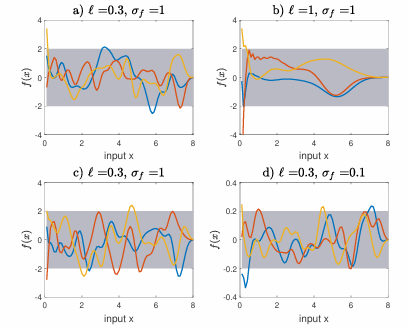
\includegraphics[width=0.65\linewidth]{figures/opt_hyp_prior.png}
    \caption{Three samples are drawn from the prior with different sets of hyperparameters. Figures (a) and (b) demonstrate the impact of changing the lengthscale, while Figures (c) and (d) illustrate the effect of varying the signal standard deviation \( f \). The uncertainty is depicted by the 95\% confidence interval, shaded in gray \cite{rezvani2019gaussian}. }
    \label{fig:opt_hyp_prior}
\end{figure}






\begin{equation}\label{eq: marginal_likelihood}
\begin{aligned}
p(w|y,X,\theta) &= \frac{p(y|X,w,\theta) \cdot p(w|\theta)}{p(y|X,\theta)}, \\
p(y|X,\theta) &= \int p(y|X,w,\theta) \cdot p(w|\theta) \, dw.
\end{aligned}
\end{equation}




The optimal solution would be a predictive distribution without dependency on the hyperparameters. By marginalization of \( \theta \), a hyperparameter-independent formalism can be obtained:

\begin{equation}\label{eq: predictive_distribution}
p(f^*|y,X,X^*) = \int p(f^*|y,\theta,X,X^*) \cdot p(y|\theta,X,X^*) \cdot p(\theta|X,X^*) \, d\theta.
\end{equation}

Unfortunately, this integral is not analytically tractable, as \( p(f^*|y,\theta,X,X^*) \) and \qquad a \( p(y|\theta,X,X^*) \) have non-trivial dependencies on \( \theta \). Several methods exist to estimate the integral, such as Hamiltonian Monte Carlo (HMC), Bayesian Monte Carlo (BMC), and Sequential Monte Carlo (SMC).

An alternative approach to approximate \eqref{eq: predictive_distribution} is by maximizing the second-level marginal likelihood (ML-II) given by \eqref{eq: marginal_likelihood}. As shown in previous work, finding the hyperparameters \( \theta_{\text{max}} \) that maximize \( p(y|X,\theta) \) leads to:

\[
p(f^*|y,X,X^*) \approx p(f^*|\theta_{\text{max}},y,X,X^*).
\]


\begin{figure}
    \centering
    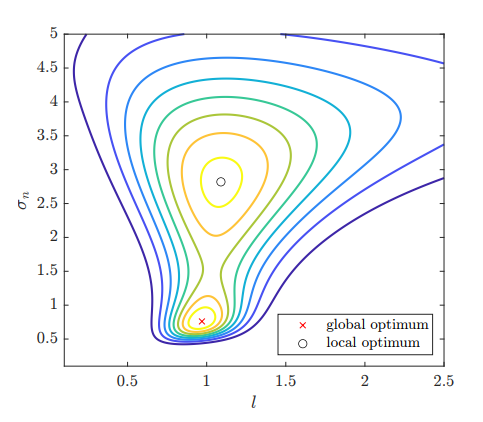
\includegraphics[width=0.75\linewidth]{figures/Contour_hyp.png}
    \caption{Contour of the marginal likelihood depending on the length scale \( l \) and noise \( \sigma_n \) \cite{Lubsen2022}.}
    \label{fig:opt_hyp_post}
\end{figure}

This method offers the advantage of analytically tractable integration. Gradient-based algorithms are typically used for maximization due to the computational efficiency of determining the partial derivatives of the likelihood with respect to \( \theta \). However, the non-convex nature of the marginal likelihood surface can lead to overfitting or underfitting. Additionally, gradient-based optimization is highly sensitive to initial values.

The contour of the marginal likelihood as a function of the length scale and noise is illustrated in Figure \ref{fig:opt_hyp_post}, showing both local and global minima. Global optimization using the hyperparameters at the global optimum results in preferable predictions compared to local minima, where observations may be misinterpreted as noise.

Reasonable hyperparameter selection is crucial, and alternative methods such as global optimizers like Dividing Rectangles (DIRECT) can be utilized to mitigate sensitivity to initial values. If the noise level is known, fixing the respective hyperparameter during optimization can prevent misinterpretation of observations.



% \begin{equation}
%     p(\theta|W,z) = \frac{p(z|W,\theta) p(\theta)}{p(z|W)}
% \end{equation}

% Here, \( p(z|W,\theta) \) is the likelihood and \( p(z|W) \) is the marginal likelihood (or evidence). However, in most cases, these integrals are intractable and numerical approximations are necessary. One approach is to maximize the likelihood \( p(z|W,\theta) \)[\cite{roberts2013gaussian}], which is effective when the likelihood is highly peaked, as is often the case with a large training dataset. A common method is to compute a point estimate of the most likely hyperparameters by maximizing the log likelihood:
% \begin{equation}
%     \log(p(z|W,\theta)) = -\frac{1}{2}z^T K^{-1} z - \frac{1}{2} \log(\text{det}(K)) - \frac{n}{2} \log(2\pi)
% \end{equation}

% with respect to \( \theta \) (see, e.g., [\cite{kocijan2016modelling}]).

% In the context of Gaussian processes (GPs), the term "learning" is used ambiguously, referring both to the inference step from prior to posterior and the optimization of hyperparameters. However, both steps are essential. GPs can be distinguished based on whether learning is performed offline or online during operation. This can involve offline inference and hyperparameter optimization [\cite{ostafew2014learning,likar2007predictive,kocijan2003predictive}], online inference and hyperparameter optimization [\cite{ortmann2017gaussian,murraysmith2003adaptive,klenske2016gaussian}], or a hybrid approach that combines offline hyperparameter optimization with online inference updates based on newly available training data [\cite{hewing2017cautious,ostafew2016learning,ostafew2014learning}]. This work considers the latter case.


% In hierarchical Bayesian models, the lowest level comprises the model parameters \( w \), given the hyperparameters \( \theta \) as introduced in Section 2.3, which define the distribution of parameters at the first level. Starting from the bottom level, the posterior over parameters is defined in (2.5) and can be expressed as
% \[
% p(w|y,X,\theta) = \frac{p(y|X,w,\theta) \cdot p(w|\theta)}{p(y|X,\theta)}
% \]
% by conditioning with \( \theta \). The denominator represents the marginal likelihood and is independent of the parameters, determined by integrating the product of the likelihood and the prior over model parameters as shown in (2.33). Ideally, the predictive distribution would be independent of the hyperparameters. However, marginalizing \( \theta \) to obtain a hyperparameter-independent formulation leads to an analytically intractable integral as shown in (2.34). Various methods, such as Hamiltonian Monte Carlo (HMC), Bayesian Monte Carlo (BMC), and Sequential Monte Carlo (SMC), can be employed to estimate this integral.

% Alternatively, approximating (2.34) can be achieved by maximizing the second-level marginal likelihood (ML-II, (2.33)). This involves finding \( \theta_{\text{max}} = \text{argmax























% The following hints are taken from the Writing-Coach, developed at the Essen University, \cite{BuBiPo00}. On that German homepage
% \begin{center}
% \href{http://www.uni-essen.de/schreibwerkstatt/trainer}
% {http://www.uni-essen.de/schreibwerkstatt/trainer}.
% \end{center} 
% much more can be found about scientific writing in German. Nevertheless lots of help in English can be found on the Internet.
% Also check out \cite{Fe13}.


% \subsection{Correctness}

% Your writing should be as accurate as possible. Do not use colloquial language, neither filler or vogue words.
% As such, technical/scientific writing style serves a purpose: to transport information as efficiently as possible.

% Respect the rules of grammar, spelling and punctuation. Text, sentences or words used in the wrong context, can 
% lead to misunderstandings or may be hard to understand. The sentences in text documents need to be complete.

% It is clear that the results of your work, e.g., experiments, are documented correctly, even though they might have had unexpected outcomes.
% Otherwise you do not only cause harm to you but any further research. 


% \subsection{Comprehensibility}

% Correctness does not imply comprehensibility. Look at your text from the readers point of view: Consider his or her position, previous knowledge
% and attitude. Formulate as precisely as possible but not more than necessary. Therefore, 
% \begin{itemize}
%     \item choose words, that are known;
%     \item use words that are probably unknown, such that their meaning can be deduced from the context, or explain or define them;
%     \item do not construct deeply nested sentences.
% \end{itemize}


% \subsection{Line of Reasoning}

% The line of reasoning depends on your topic and the type of text. To get a general structure, address the following six questions:

% \begin{enumerate}
%     \item What is the purpose of the text?
%     \item What is the content? What is to be included and why?
%     \item What is not (anymore) part of the content? What is to be excluded?
%     \item Which parts of the contents belong together? What is the structure of the topic?
%     \item What part of the contents is suited to conclude with?
%     \item What part of the contents is suited to start with?
% \end{enumerate}

% These questions show the possibilities for a line of reasoning. They show that---even for one type of text with one purpose---different lines of reasoning are possible. 
% To choose one, it is important to analyze the topic and the content.


% \subsection{References}

% One of the most important differences between scientific writing and writing other texts is citing the references used for your work. 
% Before starting to write your scientific text, you have probably been reading (or you still are) a lot of books, articles, conference proceedings, 
% manuals, etc. Some may turn out to be of no interest, but some may give you the fundamental ideas. 

% In any case, you have to cite those references you made use of and point out all parts of your work that are based on results of others 
% (those could even be your own results, if you have already published some work).

% The citation normally follows a sentence, separated by a comma. In general you don't use direct quotes in engineering sciences, but repeat the contents in your own words for better understandability
% and make clear from the proper positioning of the citation---and if necessary an additional clarifying sentence---that you are referring to other work.

% The bibliography follows at the end of your work, prior to the appendix. All your cited references are listed here. \LaTeX\ offers many ways to generate
% such a listing automatically, which will be explained in the next chapter.

% \subsection{Structure}

% Start your scientific text with an introduction, that
% \begin{itemize}
%     \item introduces the subject,
%     \item specifies the topic,
%     \item reflects on the problem that you are going to consider,
%     \item defines the purpose of the work,
%     \item explains the line of reasoning
%     \item sketches the structure of the work.
% \end{itemize}

% Keep in mind that there are some readers that only read the introduction and conclusion of your work
% and base their decision on whether the work bears any interest for them only on these parts. To make that decision,
% they need to get all relevant information from those two chapters. Hint: Look at other work with a focus on that question.

% The main part of your work should be structured as well, however here there are no general rules. The order of your
% chapters depends, if your focus was either on theoretic, methodical or experimental work. Think about a weighting for each
% chapter. What is reflected in volume and does not necessarily need to be proportional to the amount of time, you have 
% spent to solve the respective problems. Sometimes it takes one week to debug a piece of code, which nevertheless should not be explained excessively.

% Your work concludes with a summary of your results. Therefore have a look at your introduction: how you have specified the problem there and does it
% match with your results. Do not present any further results here that have been not presented in the main part. As such, always clearly
% separate the presentation and the discussion of results.

% Finally, you end with an outlook that points out open questions. What should be further analyzed and what are possible followup projects?
% Do not be afraid to point out questions that came to your mind during your research, but you did not have time to properly answer. 
% A good thesis may raise more questions than it clarifies.